\section{The ZFOURGE Survey} \label{Sec: The ZFOURGE Survey}
\subsection{Overview}

\begin{itemize}
    \item \textcolor{red}{One of my main worries regards the sample selection, which, particularly for high-redshifts and high levels of obscuration, can miss a fraction of dusty infrared sources. In fact, the near-IR bands at $z>2$ sample the optical rest-frame (UV at $z>4$), favouring the selection of dust-free objects. This is a bit at odds with the goal of deriving and decomposing the infrared luminosity function, especially because, as the authors state "the properties of Infrared (IR) light make it the ideal regime for studying SF and AGN LFs as both processes are often dusty and obscured (optically thick)." How do the authors deal with the potential incompleteness? How they account for the fraction of oscured galaxies/AGN missed by the ZFOURGE selection?}

    \item \textcolor{Green}{@Michael?}
\end{itemize}


This study utilises the 2017 release\footnote{Available for download at \href{https://zfourge.tamu.edu/}{zfourge.tamu.edu.}} of the ZFOURGE survey \citep{straatman_fourstar_2016}, which offers a unique combination of depth and wavelength coverage essential for probing high-redshift galaxies and constructing accurate LFs. ZFOURGE consists of approximately 70,000 galaxies at redshifts greater than 0.1 covering three major 11$\times$11 arcminute fields: the Chandra Deep Field South (CDFS) \citep{giacconi_chandra_2002}, the field observed by the Cosmic Evolution Survey (COSMOS) \citep{scoville_cosmic_2007}, and the CANDELS Ultra Deep Survey (UDS) \citep{lawrence_ukirt_2007}. These galaxies were observed using the near-infrared FourStar imager \citep{persson_fourstar_2013} mounted on the 6.5-m Magellan Baade Telescope at the Las Campanas Observatory in Chile. 

ZFOURGE employs deep near-infrared imaging with multiple medium-band filters (\textit{J}$_{1}$, \textit{J}$_2$, \textit{J}$_{3}$, \textit{H}$_{l}$, \textit{H}$_{s}$) and a broad-band \textit{K}$_{s}$ filter. The imaging spans 1.0 to 1.8 $\mu$m and achieves 5$\sigma$ point-source limiting depths of 26 AB mag in the \textit{J} medium-bands and 25 AB mag in the \textit{H} and \textit{K}$_{s}$ bands \citep{spitler_first_2012}. These filters yield well-constrained photometric redshifts, particularly effective for sources within the redshift range of 1 to 4 \citep{spitler_first_2012}. ZFOURGE data is supplemented by public data from HST/WFC3 F160W and F125W imaging from the CANDELS survey, Spitzer/Infrared Array Camera (IRAC), and Herschel/Photodetector Array Camera and Spectrometer (PACS). For a detailed description of the data and methodology, refer to \cite{straatman_fourstar_2016}.

\subsection{Sample Selection} \label{Sec: Sample Selection}
\begin{itemize}
    \item \textcolor{red}{I do not agree with the removal of sources with "unphysical bolometric luminosities": How was their bolometric luminosity obtained? Is it IR bolometric, or does it include also X-ray, UV, optical and radio? Is AGN bolometric + galaxy bolometric? Why not keeping all the sources without introducing an unnecessary incompleteness in the sample, and recompute their bolometric luminosities using the CIGALE SED-fitting?}
    
    \item \textcolor{Green}{Based upon the reviewer's comments throughout the paper, it has come to our attention that certain aspects of our paper were poorly explained (which we have now improved). The luminosity for ZFOURGE and CIGALE sources are calculated with separate methods. ZFOURGE uses the singular average Wuyts template based on the 24um flux whereas CIGALE has potentially thousands of templates to compare against. We do not expect the ZFOURGE total to be the sum of the CIGALE AGN and SF components; that role would be fulfilled by a CIGALE total LF. However, we deemed the CIGALE total LF to be unnecessary because it is almost exactly the same as the CIGALE Stellar, which is much more interesting. We performed the SED decomposition with CIGALE on all sources, regardless if they were later removed from the CIGALE LF sample. Our original intention was to present LFs as they have been in the past, as well as include an updated method utilising SED decomposition so that the reader may choose which is most suitable for them to utilise in their own work. We intended to present the CIGALE LFs using the sample of ZFOURGE sources, which were not reduced according to the sample reduction, in order to present the LFs as closely to each other as possible. We realise this has negatively impacted the CIGALE LF and so now we utilise the entire available sample. We realise that the presentation and description were not as clear as we had hoped, so we now resubmit this revised manuscript to the reviewer.
    \begin{itemize}
        \item Are these sources real negative luminosities, or are they just upper/lower limits?
        \item We believe it would not be a fair representation of the original ZFOURGE LF if we were to recalculate the total luminosity using CIGALE.
        \item address incompleteness: ejecting dim/negative luminosity sources inherently happens based on the luminosity bins. "This does not affect the completeness of the sample" at "we refine..." 
    \end{itemize}
    }
\end{itemize}

\subsubsection{ZFOURGE total \sout{\& Decomposed SF} Sample} \label{Sec: Galaxy LF Selection}
To ensure the selection of high-quality galaxies and minimise errors in our analysis, we adopt the ZFOURGE quality flag \texttt{Use=1}, as defined by \cite{straatman_fourstar_2016}. This flag selects galaxies with reliable photometry and redshift measurements, resulting in a starting sample of 37,647 galaxies. We refine the sample by removing sources with \textcolor{red}{poorly constrained/undetermined} bolometric luminosities (labelled $L_{bol} < 0$), which reduces the sample to 22,997 galaxies.

\sout{Next, we use the ZFOURGE AGN catalogues to identify and exclude 552 AGN-dominated sources to prevent AGN contamination of the luminosity functions. After excluding these AGN sources,} We apply a redshift cut, restricting the sample to $0 \leq z \leq 6$ since only 28 galaxies exist at $z > 6$ (yielding  22,967 galaxies). This redshift range enables us to observe the evolution of galaxies during some of the most critical cosmic periods, specifically around $1 < z < 3$ \citep{gruppioni_modelling_2011, wylezalek_galaxy_2014} where galaxy luminosity density peaks \citep{assef_mid-ir-_2011}.

To ensure robustness, we calculate the bolometric flux from the bolometric luminosity of each sample and apply an 80\% completeness cut. This reduces the impact of noise and observational limits while preserving a large enough sample for LF construction. The final ZFOURGE total sample includes 18,373 galaxies. \sout{We also apply a completeness cut that requires the maximum observable volume of each galaxy to extend to the end of the redshift bin. These completeness cuts reduce the final LF sample to 16,154 galaxies.}

Editor:
\begin{itemize}
    \item \textcolor{red}{It is not clear from the text whether and how the selection biases have been taken into account. In particular, it is not clear how the rejection of ~14000 objects with negative Lbol measurements affects the completeness of the sample.}
    \item \textcolor{Green}{These sources have negative luminosities. They cannot be used in the luminosity function. Perhaps look into how the original Lbol values were calculated?}
    \vspace{0.25cm}

    \item \textcolor{red}{The exclusion of the AGN-dominated object also needs some motivation, and given that the definition of "AGN-dominated" is very often wavelength dependent, further information about what exactly has been excluded and why is needed.}
    \item \textcolor{Green}{552 "AGN dominated" sources were originally removed from the ZFOURGE total and CIGALE SF because we did not want to introduce an AGN component into our star-forming sample. However, we realise this has introduced a potential bias, so we have re-added the AGN component into the ZFOURGE total (to be more 'total") and CIGALE SF (trusting CIGALE to do the decomposition).}
    \vspace{0.25cm}
    
    \item \textcolor{red}{Furthermore, it is unclear from the text (one needs to look in Straatman+16 for the information) what fraction of the catalogue has coverage at PACS 160 micron. long wavelength data are necessary to better constraint the dust heated by star formation in the SED fit.}
    \item \textcolor{Green}{As far as I know, there is minimal, if not zero usage of PACS 160 in the ZFOURGE dataset we use. Need to justify why this is not a bad thing. I seem to remember that the 24um is adequate and estimates the far-IR quite well?}
    \vspace{0.25cm}
    
    \item \textcolor{red}{ I would therefore like to invite the authors to briefly discuss the photometry available for the full catalogue, address the issue of possible lack of strong constraints in the far infrared (if indeed an issue), as well as the inaccuracies or uncertainties this may lead to in the revised version.}
    \item \textcolor{Green}{Okay, add a few sentences discussing}
    \vspace{0.25cm}
\end{itemize}

Reviewer:
\begin{itemize}
    \item \textcolor{red}{My main concerns are mostly related to the sample selection and incompleteness, to the different functional forms used for different components, and to the inconsistent results obtained for the total and splitted LFs. The incompleteness, present in the original sample, and also introduced by the exclusion of sources during the analysis, is neither taken into account in the calculation, or discussed in the text.}
    
    \item \textcolor{red}{I do not understand the reason why the ZFOURGE AGN are excluded from the analysis. Even if they are AGN-dominated sources, they can still contain a significant amount of star formation (see, i.e., Hatziminaoglou et al. 2010). Therefore, the SED decompositions should be applied also to them, and the resulting AGN and SF components should be used in the analysis.}
    \item \textcolor{Green}{I will include AGN dominated for CIGALE SF as the SF component will still contribute and AGN is minimised inherently. Should AGN be included for ZFOURGE? Perhaps it should if it is the "total". Lucky we already have the decomposed components and do not need to rerun CIGALE.}
    \vspace{0.25cm}
    
    \item \textcolor{red}{What does it mean "to prevent AGN contamination", when the goal is to obtain complete AGN and SF LF functions? The sample is potentially incomplete due to the near-IR selection, why adding further incompleteness by excluding pre-classified AGN?}
    \item \textcolor{Green}{The original intent was to provide a SF LF with AGN "contamination" minimised, in the same way providing an AGN LF with SF "contamination" minimised. I see how the reviewer could confuse this and will improve the description.}
    \vspace{0.25cm}
    
    \item \textcolor{red}{If the authors trust their decomposition analysis, they should apply it to *ALL* the sources in the sample.}
    \item \textcolor{Green}{As above, this will not provide a good comparison. There would be far more SF and AGN components than ZFOURGE, unless recomputing the ZFOURGE Lbol}
    \vspace{0.25cm}
    
    \item \textcolor{red}{What does it mean "bolometric flux"? How is calculated? Is it derived in each band? How? Please, specify. Also the way the bolometric luminosity has been obtained should be explained.}
    \item \textcolor{Green}{Flux as defined by the luminosity-distance relationship: $F=L/4\pi d^2_L$. The bolometric flux is calculated for each ZF total, CIGALE SF and AGN. Perhaps this is unnecessary? Describe why done if kept.}
    \vspace{0.25cm}
    
    \item \textcolor{red}{Is it really necessary to exclude sources due to their volume not reaching the accessible volume in the z-bin? Why not simply weight each galaxy for its max volume obtained from the minimum between the z-bin max accessible volume and the max accessible volume due to their luminosity?}
    \item \textcolor{Green}{I have worded this poorly. What I have actually done is use the luminosity distance to create another "cut". This has the effect of limiting the sample to sources with both luminosity distance and comoving distance above a certain limit. The primary outcome of this is that it serves as the "completeness limit"  on the LF, where after which the LF would turn over without this in place. A secondary effect is that it removes sources with maximum distances that do not extend to the end of the redshift bin. In essence, it makes no difference because these sources only appear after the "turn over" or inside the incomplete region.}
    \vspace{0.25cm}
\end{itemize}

\subsubsection{Decomposed Sample} \label{Sec: Decomposed AGN Selection}

\begin{itemize}
    \item \textcolor{red}{How are the previously excluded AGN treated in the AGN sample decomposition with CIGALE? Are they considered as powered only by AGN, or are they decomposed together with the other sources? I do not understand why the two samples (AGN and SF galaxies) are defined before performing the SED fitting and decomposition: shouldn't be the CIGALE decomposition to define the two samples? This part is not clear and should be more extensively described.}
    \item \textcolor{Green}{perhaps moving section 3 to appear before section 2?}
\end{itemize}

\sout{Although AGN-dominated sources are removed from the ZFOURGE galaxy and CIGALE SF sample, they are retained for separate analysis to construct decomposed AGN LFs through SED decomposition.} The SF and AGN components are decomposed using the \texttt{CIGALE} software. For a comprehensive explanation of the SED decomposition process, please refer to Section \ref{Sec: CIGALE}. We continue to apply the ZFOURGE survey's \texttt{Use=1} for our analysis, as well as removing failed fits, resulting in an initial sample of 37,574 sources. For our AGN-specific analysis, we include all sources with a significant AGN fraction ($\mathcal{F}_{AGN}>0.1\ L_{AGN}/L_{bol}$); 21,063 sources. After applying the same 80\% completeness cut to the bolometric flux, the AGN and SF sample is reduced to a final set of 16,850 and 30,059 sources, respectively, spanning $0 \leq z \leq 6$. Figure \ref{Fig: ZF Lum vs z} shows the reduced luminosity-redshift distribution of ZFOURGE (top), CIGALE AGN (middle), and CIGALE SF (bottom).

\textcolor{red}{there is no use flag in our cigale sample, so we continue to use zfourge use to keep a consistent number density and remove stars, bad sources, etc}

\begin{figure}
    \centering
    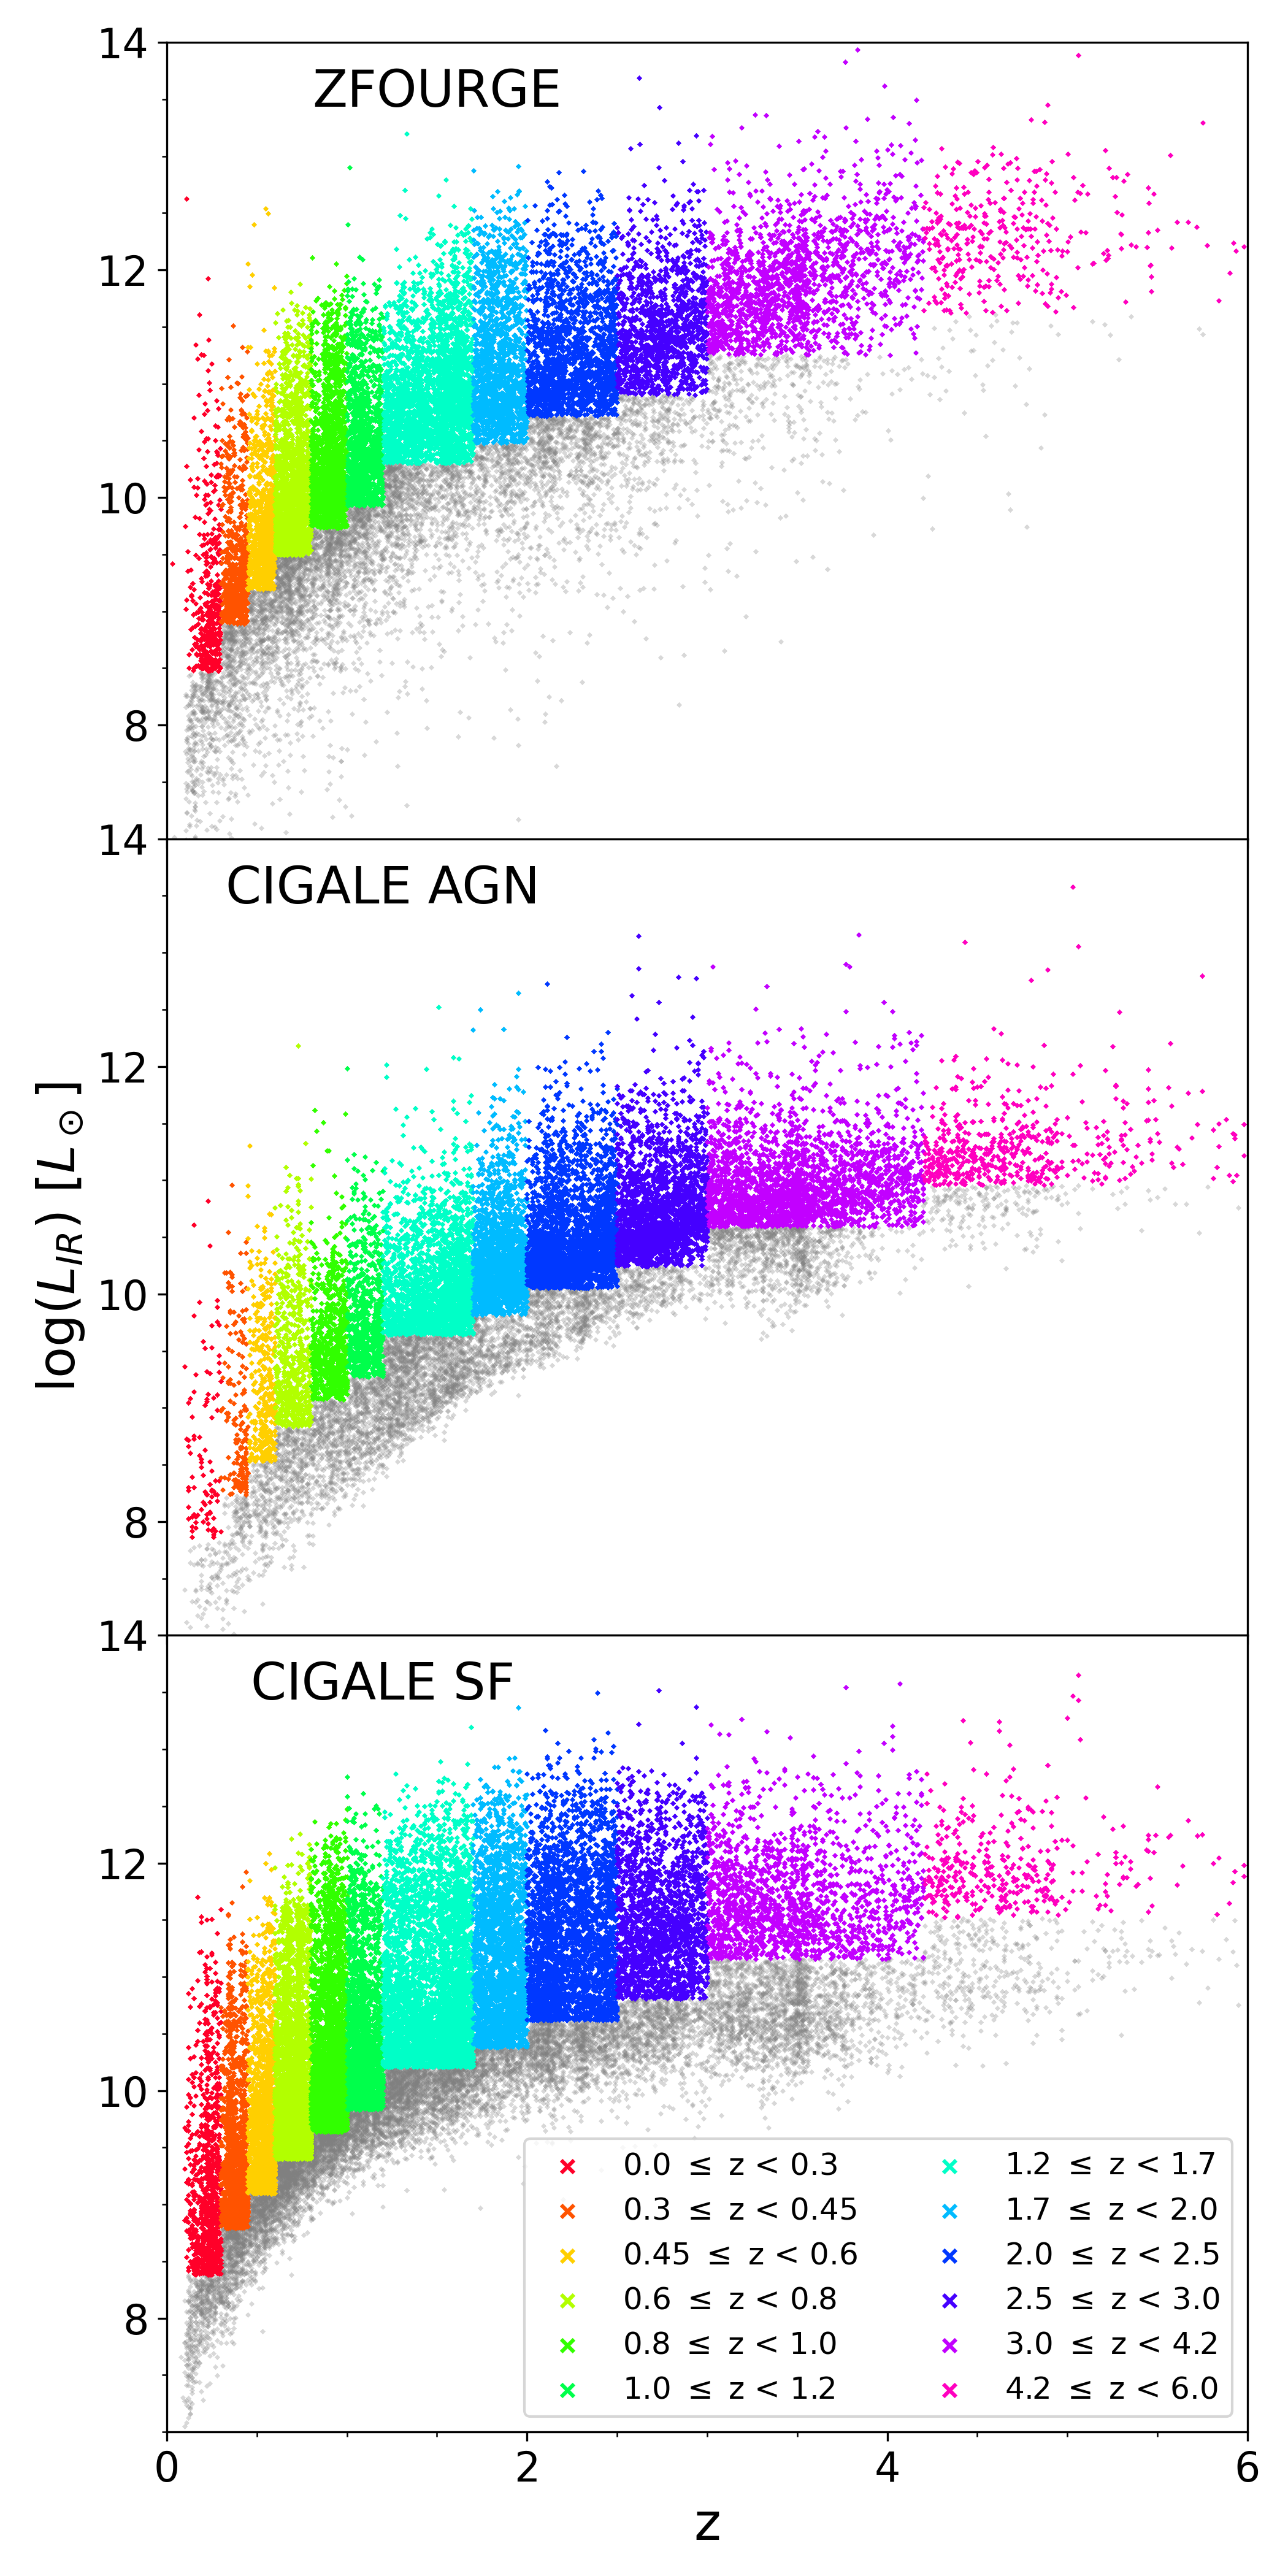
\includegraphics[width=0.48\textwidth]{Figures/LIR_vs_Z.png}
    \caption{Luminosity-redshift distributions of (top) the ZFOURGE bolometric $8-1000\mu m$ luminosity, (middle) the CIGALE AGN luminosity, and (bottom) the CIGALE SF luminosity. Sources are coloured by redshift bin or coloured grey if removed as described in section \ref{Sec: Sample Selection}}
    \label{Fig: ZF Lum vs z}
\end{figure}

% \textcolor{red}{is this paragraph even necessary? I feel like it could be deleted entirely.} We use the UVJ colour-colour diagram to differentiate between quiescent and star-forming galaxies by selecting a quiescent galaxy mask with equation \ref{EQ: UVJ} \citep{cowley_zfourge_2016}. \textcolor{red}{better reference?}. Where U, V, \& J are the rest-frame Johnson U, V and 2MASS J filters respectively. \citep{straatman_fourstar_2016}. Star-forming galaxies are selected by taking the inverse of the quiescent galaxy mask.

% \begin{equation}
%     \label{EQ: UVJ}
%     \begin{split}
%         & U-V > 1.3, \\
%         & V-J < 1.6, \\
%         & U-V > 0.88 \times (V-J) + 0.59
%     \end{split}
% \end{equation}